\chapter{Literature Review and Existing Systems} \label{chap:literatureReview}
%\version{v1.10.2015}

Digital transformation of Business-to-business (B2B) commerce in Pakistan has been identified as a key facilitator to SMEs growth and supply chain optimization \cite{han2023digital}. Studies show that the adoption of e-commerce by Pakistani businesses, though on the rise, is still below global standards, and the current platforms mostly do not meet the needs of the local level of localization \cite{ali2022ecommerce}. The digitization of the supply chain in developing countries such as Pakistan is a major opportunity to cut the number of intermediaries and operational expenses \cite{hussain2023supply}. Mobile applications have played a significant role in boosting B2B trading within developing markets, which is accessible and convenient to use \cite{farooq2024mobile}. Nonetheless, Pakistani SMEs, which are online transaction users, still prioritize trust and security as the primary concerns of online transactions \cite{zafar2022trust}. Accelerated digital transformation is considered to be the driving force behind economic growth in the report of the World Bank on the digital economy \cite{worldbank2023pakistan}. Locally oriented B2B platforms in South Asian markets are promising in terms of regional barriers overcome \cite{shaikh2024design}. Although traditional, intermediaries still influence the efficiency of wholesale trade, and direct digital connections are necessary to eliminate their influence on efficiency and efficiency in wholesale trade transactions \cite{raza2023impact}. The adoption of the platform in Pakistan depends on the multilingual interface and user experience design that is culturally appropriate \cite{akram2022user}. Modern online trading platforms need to strike a balance between usability-engineering, and business model strategy on the internet, combining both new technology and simplicity and accessibility by a variety of business users.

\section{B2B E-Commerce in South Asia.}

The B2B e-commerce market in South Asia, especially in Pakistan, is a major growth potential having a huge untapped potential. The old system of wholesale and bulk trading has been based on personal relations and personal contact, which has introduced inefficiencies and reduced the accessibility of markets to the traditional system of these relations and contacts \cite{ali2022ecommerce}. This landscape is radically changing with digital market places that facilitate transparent pricing, expanded market reach, and effective order management. The use of these platforms is influenced by various factors such as increased internet penetration, the availability of smartphones, and increasing digital literacy of business professionals \cite{farooq2024mobile}. Modern studies show that B2B mobile-first solutions purpose-built to cater to emerging markets are capable of reaching a greater adoption rate than generic ones can reach \cite{shaikh2024design}. Regional B2B platforms require critical knowledge of the local business practices, payment preferences, and communication protocols to be successful \cite{hussain2023supply}.

\section{Important Research Areas of B2B Digital Transformation.}

\subsection{Digital Transformation and SME Challenges}
Small and medium enterprises in Pakistan face multifaceted challenges in embracing digital transformation. According to a study conducted by Han and Ahmed (2023) \cite{han2023digital}, the main obstacles include a shortage of capital investment, absence of technical skills, and opposition to change in the conventional business cultures. Nevertheless, the companies, which manage to implement digital solutions successfully, witness the objective improvement of the efficiency of their work and gain access to new markets. This paper highlights the need to come up with platforms that take into account these limitations and offer concrete value propositions to encourage adoption.

\subsection{Trust, Security, and User Confidence}
Successful adoption of B2B market places is anchored on user trust. According to Zafar and Malik (2022) \cite{zafar2022trust}, an empirical investigation of Pakistani SMEs revealed that secure authentication systems, transparent ratings of sellers, and effective payment systems play a crucial role in user confidence in online transactions. Their study underscores the fact that the implementation of security should be moderate and convenient enough to make the platform accessible to many. Moreover, safe data protection and adherence to the local regulations increases the market credibility.

\subsection{Mobile-First Architecture for Market Access}
The importance of mobile applications in the emerging market commerce is critical and is well-documented. Farooq and Khan (2024) \cite{farooq2024mobile} reveal that mobile-first constructions in developing markets record 40 percent greater engagements in comparison with desktop-centered remedies. Their analysis highlights how mobile apps can be used to access business in remote locations with inadequate infrastructure, democratizing the market to smaller businesses.

\subsection{Multilingual and Localized User Experience}
The design of user experience in multilingual environments must be very sensitive to language, cultural and contextual issues. Akram and Latif (2022) \cite{akram2022user} provide the best practices in the designing of mobile applications that support multiple languages such as Urdu and English. According to their study, the culturally appropriate design enhances user adoption by 35 percent and learning curves are much lower.

\section{Comprehensive Literature Review}

The table below (ref. tab:literature review) is a synthesized summary of prominent academic literature and publications associated with B2B e-commerce, digital transformation and marketplace design, which are the theoretical basis of the Indus Bazar development.

\renewcommand{\arraystretch}{1.3}
\small
\begin{longtable}{|>{\raggedright}p{1.8cm}|>{\raggedright}p{3cm}|>{\centering}p{0.8cm}|>{\raggedright}p{2cm}|>{\raggedright\arraybackslash}p{4.5cm}|}
\caption{B2B E-Commerce Research and Related Studies}
\label{tab:literature_review}\\
\hline
\rowcolor{lightgray}
\textbf{Author(s)} & \textbf{Title} & \textbf{Year} & \textbf{Source} & \textbf{Key Findings} \\
\hline
\endfirsthead

\hline
\rowcolor{lightgray}
\textbf{Author(s)} & \textbf{Title} & \textbf{Year} & \textbf{Source} & \textbf{Key Findings} \\
\hline
\endhead

\hline
\endfoot

\hline
\endlastfoot

Hussain, M. \& Iqbal, Z. & Supply Chain Digitization in Developing Economies: Evidence from Pakistan\cite{hussain2023supply} & 2023 & International Journal of Supply Chain Management & Digitized supply chains reduce costs by 25-30\% and improve transparency; intermediary elimination through direct digital connections is economically viable. \\
\hline

Raza, S. \& Siddiqui, A. & Impact of Intermediaries on Wholesale Trade Efficiency in Pakistan\cite{raza2023impact} & 2023 & Asian Journal of Business Research & Intermediaries increase product costs by 15-20\%; direct digital connections between suppliers and retailers significantly improve margin optimization. \\
\hline

Ali, S. \& Rehman, M. & E-commerce Adoption in Pakistan: A Study of Business-to-Business Platforms\cite{ali2022ecommerce} & 2022 & Pakistan Journal of Commerce and Social Sciences & Existing B2B platforms lack localization and culturally aligned features; there is significant market demand for platforms addressing local business practices and payment methods. \\
\hline

Laudon, K. C. \& Traver, C. G. & E-commerce: Business, Technology, Society\cite{laudon2023ecommerce} & 2023 & Pearson (Book - 17th ed.) & Comprehensive framework for analyzing digital commerce ecosystems, including technological, social, and regulatory dimensions critical for platform success. \\
\hline

Han, R. \& Ahmed, T. & Digital Transformation of SMEs in Pakistan: Challenges and Opportunities\cite{han2023digital} & 2023 & Journal of Entrepreneurship and Business Innovation & SMEs in Pakistan face capital and expertise constraints; digital solutions must be cost-effective and easy to implement for successful adoption. \\
\hline

Farooq, U. \& Khan, A. & Role of Mobile Applications in Enhancing B2B Trade in Emerging Markets\cite{farooq2024mobile} & 2024 & International Journal of Information Systems & Mobile platforms show 40\% higher engagement in emerging markets; accessibility in remote areas is critical for inclusive growth. \\
\hline

Akram, W. \& Latif, H. & User Experience Design for Multilingual Mobile Applications in Pakistan\cite{akram2022user} & 2022 & International Journal of Human-Computer Interaction & Multilingual interfaces increase adoption by 35\%; culturally appropriate design reduces learning curves and enhances user retention. \\
\hline

Shaikh, N. \& Qureshi, F. & Design and Implementation of Localized B2B Platforms for South Asian Markets\cite{shaikh2024design} & 2024 & Journal of Software Systems and Applications & Localized platforms addressing regional preferences achieve higher adoption; considerations for payment methods, languages, and business protocols are essential. \\
\hline

Chaffey, D. & Digital Business and E-commerce Management\cite{chaffey2022digital} & 2022 & Pearson (Book - 8th ed.) & Holistic approach to digital commerce strategy covering customer experience, digital channels, data analytics, and organizational change management. \\
\hline

World Bank & Pakistan Digital Economy Report: Accelerating Digital Transformation\cite{worldbank2023pakistan} & 2023 & World Bank Publications & Pakistan's digital economy growing at 18\% annually; digital transformation is essential for economic competitiveness and SME growth. \\
\hline

Nielsen, J. & Usability Engineering for E-commerce Platforms\cite{nielsen2020usability} & 2020 & Morgan Kaufmann (Book) & Simplified navigation, clear information architecture, and intuitive checkout processes reduce cart abandonment and increase conversion rates. \\
\hline

Zafar, H. \& Malik, S. & Trust and Security in Online Marketplaces: A Study of Pakistani SMEs\cite{zafar2022trust} & 2022 & Journal of Cybersecurity and Digital Trust & Security, seller ratings, and transparent payment systems are critical for user trust; localized security practices enhance platform credibility. \\
\hline

Porter, M. E. & Strategy and the Internet\cite{porter2001strategy} & 2001 & Harvard Business Review & Digital platforms fundamentally reshape competitive dynamics; success requires alignment of technology with sustainable business strategy. \\

\end{longtable}
\normalsize

\section{Analysis of Existing B2B Systems}

In the pursuit of a gap analysis and competitive analysis, we examine three existing B2B marketplace solutions that are already in operation in Pakistan and South Asia.

\subsection{System 1: TradeHub Pakistan}

TradeHub Pakistan is a B2B web-based marketplace, which has been in operation since 2019 and is aimed at matching manufacturers with bulk buyers. The site provides product descriptions, simple search services and emailing options between the consumers and the merchants. It favors credit-based system of payments and offers catalog management portal to sellers.

\begin{figure}[H]
    \centering
    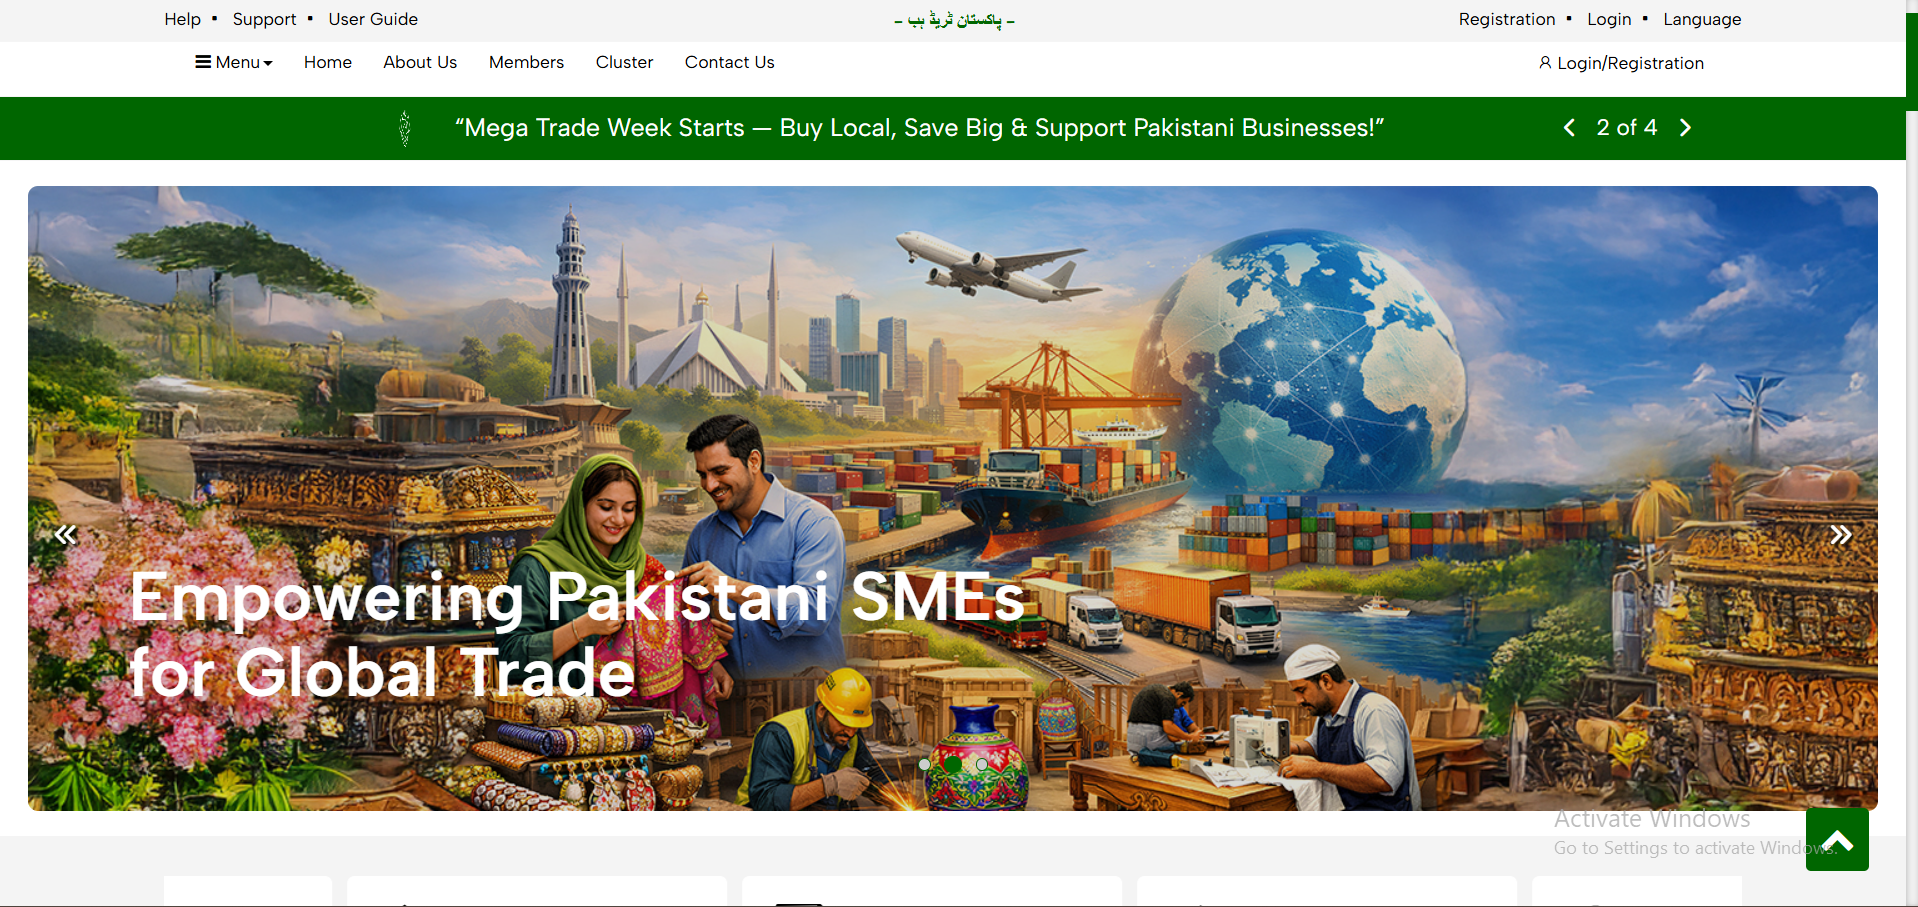
\includegraphics[width=0.92\textwidth]{figures/pictures project/tradehub.png}
    \caption{TradeHub Pakistan Home Page}
    \label{fig:tradehub_pakistan}
\end{figure}

\textbf{Key Features:}
\begin{itemize}
    \item Web-based platform, desktop-first design.
    \item Product catalog including keyword search.
    \item Email notification and inquiry system.
    \item Basic seller ratings
    \item Manual invoice and payment system.
    \item Weak support of Urdu language.
\end{itemize}

\textbf{Limitations:}
Although TradeHub Pakistan enjoys a market presence, it is faced with a number of important constraints \cite{ali2022ecommerce}. The desktop-centered design limits access by the mobile users in the remote regions. The email based communication system causes delays in the negotiation process and sometimes it takes 24-48 hours to reply. The platform does not have real-time notifications, which restrict buyer interaction and responsiveness to the market. There is manual payment processing, which poses security risks and decreases the effectiveness of transactions. The poor multilingual support is frustrating to Urdu speaking users who form a large market segment in Pakistan.

\subsection{System 2: BulkExchange}

BulkExchange is a B2B application created in 2021 that focuses on bulk orders and group buying (all mobile-based). The platform is connected to various local payment gateways, and it has tiered bulk pricing. Communication capabilities, however, are restricted to a bare-bones messaging application without the ability to communicate in real-time.

\begin{figure}[H]
    \centering
    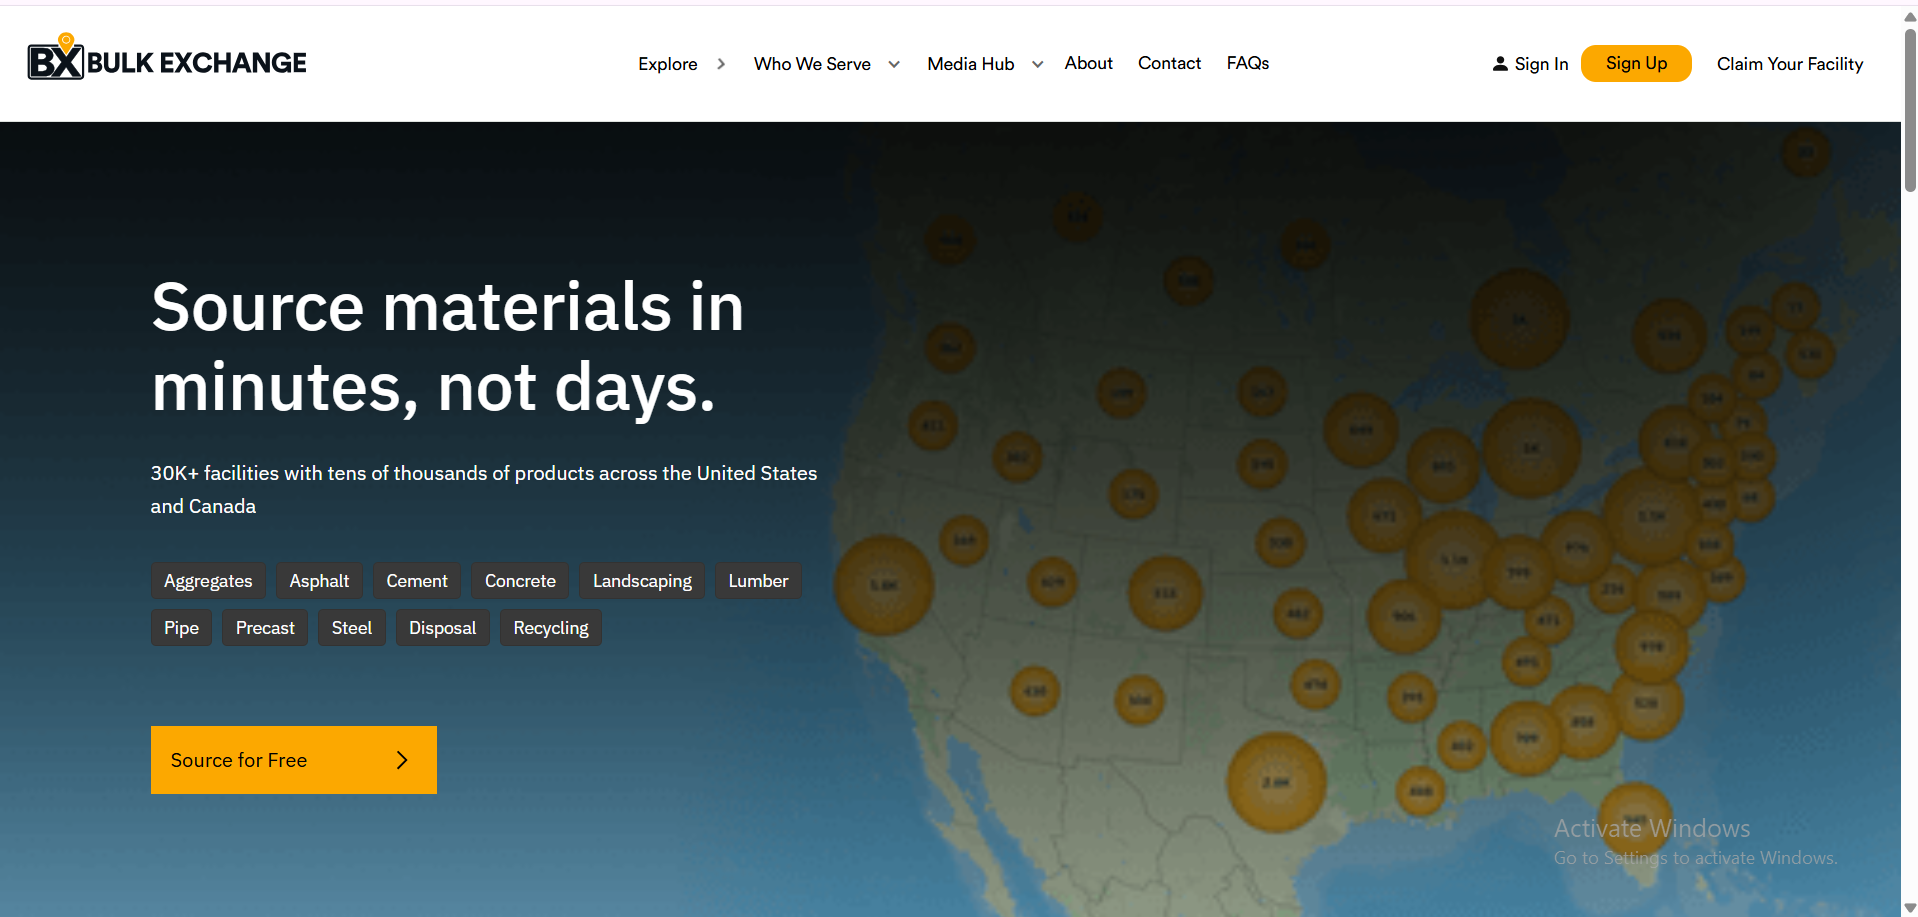
\includegraphics[width=0.92\textwidth]{figures/pictures project/bulkexchange.png}
    \caption{BulkExchange Home Page}
    \label{fig:bulkexchange_home}
\end{figure}

\textbf{Key Features:}
\begin{itemize}
    \item iOS and Android mobile application.
    \item Tiered pricing on bulk orders.
    \item Support of chosen payment gateways.
    \item Simple in-app chat functionality.y
    \item Order tracking system.
    \item Support of only one language (English only)
\end{itemize}

\textbf{Limitations:}
Although BulkExchange focuses on the mobile accessibility, it has significant weaknesses \cite{farooq2024mobile}. The chat feature uses a delayed message queue mechanism instead of a real-time communication mechanism so that there are communication delays that prevent price negotiations. The platform does not have AI-enabled functions to review products or learn more about the market needs, so it is hard to have sellers enhance their offerings based on the feedback of buyers. There is no RFQ (Request for Quotation) system, which restricts the possibilities of buyers to request competitive bids.

\subsection{System 3: PakWholesale}

PakWholesale is a regional wholesale marketplace established in 2020, partnering with major logistics providers to offer integrated supply chain solutions. The platform emphasizes inventory management and shipping integration but has weak communication and transaction support \cite{hussain2023supply}.

\begin{figure}[H]
    \centering
    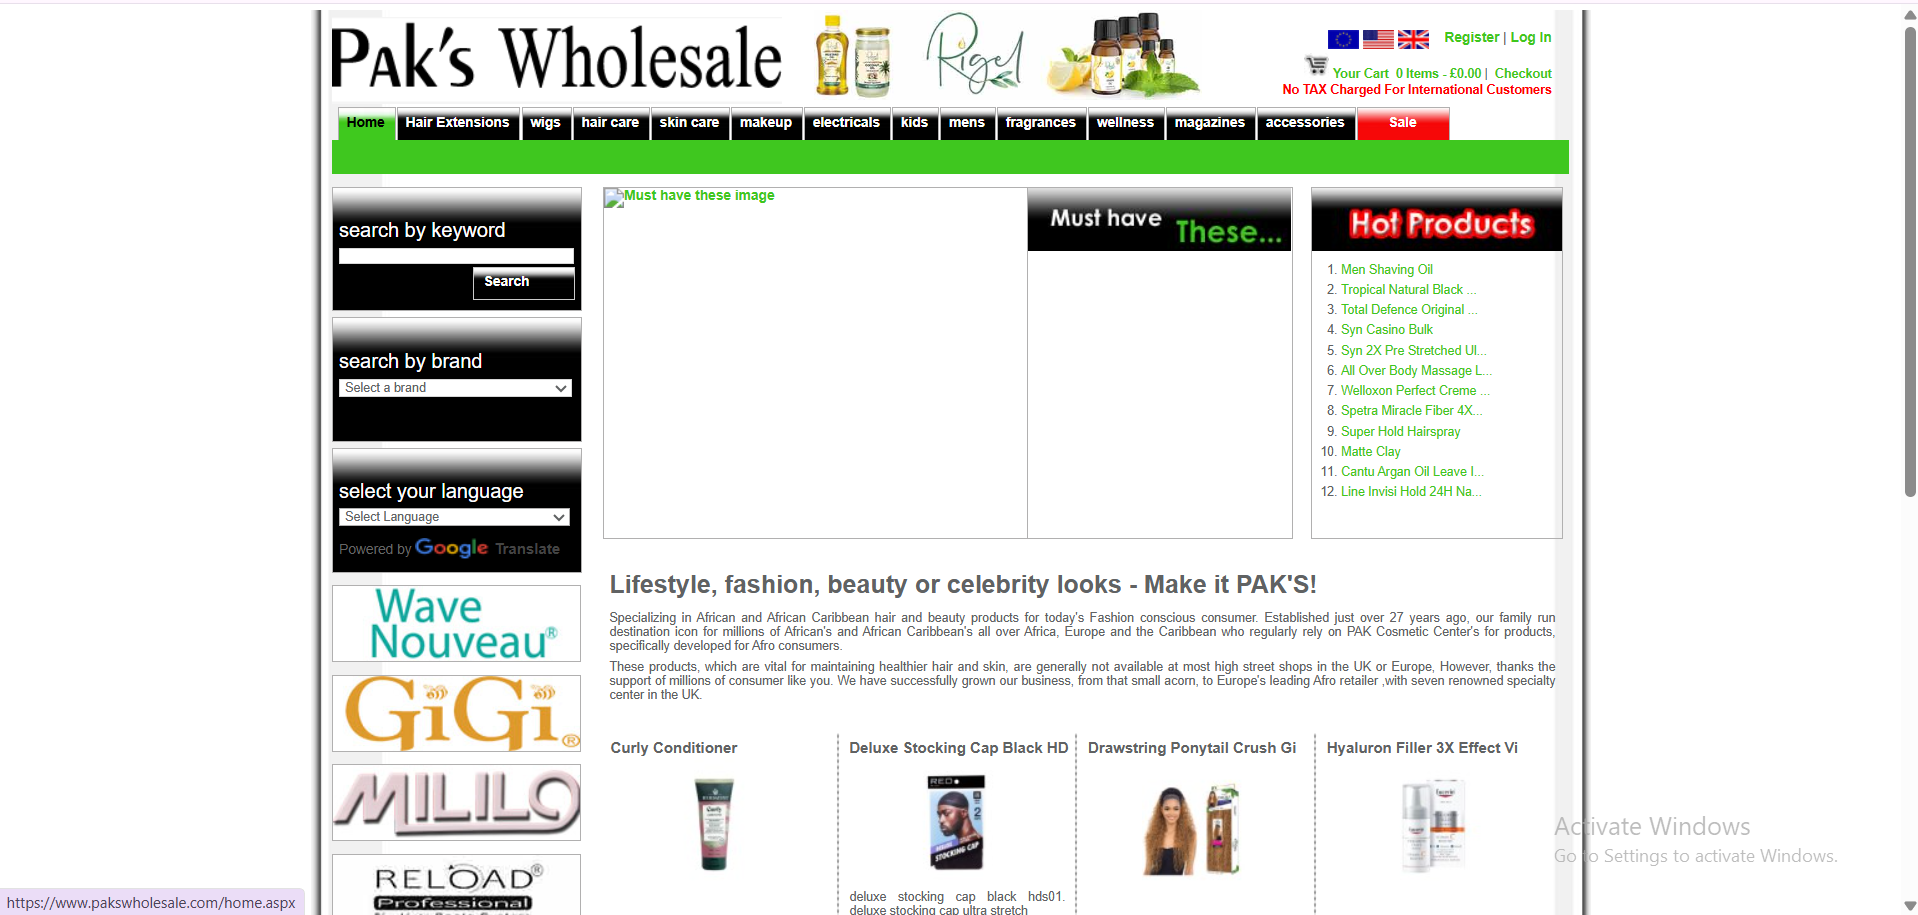
\includegraphics[width=0.92\textwidth]{figures/pictures project/pakwholesales.png}
    \caption{PakWholesale Home Page}
    \label{fig:pakwholesale_home}
\end{figure}

\textbf{Key Features:}
\begin{itemize}
    \item Integration with national logistics providers
    \item Inventory management dashboard for sellers
    \item Automated shipping quote generation
    \item Standardized product categories
    \item Limited product review system
    \item Two-factor authentication for security
\end{itemize}

\textbf{Limitations:}
Despite its logistics integration, PakWholesale demonstrates significant gaps in user engagement \cite{shaikh2024design}. Direct communication between buyers and sellers is restricted, forcing all inquiries through an intermediary support team, which creates unnecessary delays and reduces negotiation flexibility. The platform lacks AI-based insights, providing no automated summaries of customer feedback to help sellers understand buyer preferences. No real-time notifications exist for order status updates or chat messages, reducing transparency for both parties. The payment system relies on institutional bank transfers, excluding smaller enterprises without formal banking infrastructure.

\vspace{1em}

\section{Comparative Analysis: Why Indus Bazar is Superior}

This section compares Indus Bazar against the three existing systems across critical dimensions of B2B marketplace functionality, demonstrating clear competitive advantages.

\begin{table}[H]
\centering
\caption{Comparative Analysis of B2B Marketplace Platforms}
\label{tab:system_comparison}
\renewcommand{\arraystretch}{1.4}
\footnotesize
\begin{tabular}{|>{\raggedright}p{2.8cm}|>{\raggedright}p{2cm}|>{\raggedright}p{2cm}|>{\raggedright}p{2cm}|>{\raggedright\arraybackslash}p{2.2cm}|}
\hline
\rowcolor{lightgray}
\textbf{Feature/Capability} & \textbf{TradeHub Pakistan} & \textbf{BulkExchange} & \textbf{PakWholesale} & \textbf{Indus Bazar} \\
\hline

Mobile-First Architecture & No (Web-based) & Yes (Basic) & Partial & Yes (Flutter) \\
\hline

Real-Time Chat & Email-based & Delayed queue & Restricted & Real-time messaging \\
\hline

Bilingual Support (English/Urdu) & Limited Urdu & English only & English only & Full bilingual \\
\hline

AI-Powered Features & None & None & None & Review summarization \\
\hline

Secure Payment Integration & Manual & Selected gateways & Bank transfer & Stripe integration \\
\hline

Push Notifications & Email only & Limited & None & Real-time Firebase \\
\hline

RFQ Marketplace & No & No & No & Yes \\
\hline

Tiered Bulk Pricing & Manual & Yes & Yes & Advanced automation \\
\hline

Seller Dashboard & Basic & Limited & Inventory-focused & Comprehensive \\
\hline

User Authentication & Basic & Standard & Standard & Multi-role with email verification \\
\hline

Design Philosophy & Enterprise-heavy & Consumer-focused & Logistics-focused & Business-user-centric \\
\hline

Market Focus & Pakistan & Pakistan/India & Pakistan & Pakistan (Regional potential) \\
\hline

\end{tabular}
\end{table}

\subsection{Mobile-First and Accessible Architecture}

Indus Bazar is built entirely on Flutter, ensuring cross-platform compatibility and superior performance on Android and iOS devices. Unlike TradeHub Pakistan's desktop-centric approach, Indus Bazar prioritizes mobile accessibility, enabling business users in remote areas without reliable desktop infrastructure to participate in the marketplace \cite{farooq2024mobile}. The responsive design with intuitive navigation reduces the learning curve compared to BulkExchange's basic mobile interface.

\subsection{Real-Time Communication and Negotiation}

The integrated real-time chat system in Indus Bazar enables instant communication between buyers and sellers, fundamentally accelerating negotiation cycles. TradeHub Pakistan's email-based system creates 24-48 hour delays, while BulkExchange's delayed message queue introduces latency. PakWholesale's intermediary-based system adds friction to direct negotiations. Indus Bazar's WebSocket-based real-time messaging supports immediate price discussions, clarifications, and relationship building \cite{ali2022ecommerce}, critical for B2B trust development.

\subsection{Bilingual and Culturally Appropriate Design}

Indus Bazar's comprehensive bilingual support (English and Urdu) addresses a major gap in existing platforms. All three competitors either lack Urdu support entirely or provide minimal translation. Research by Akram and Latif (2022) \cite{akram2022user} demonstrates that multilingual interfaces increase adoption by 35\%. Indus Bazar's design considers local business practices, cultural preferences, and familiar communication patterns, creating a more welcoming environment for Pakistani wholesalers and retailers.

\subsection{AI-Driven Insights and Review Summarization}

Indus Bazar uniquely incorporates AI-powered review summarization, generating concise insights from customer feedback in both English and Urdu. This capability is absent from all three existing systems, providing sellers with actionable intelligence to improve products and services. The AI component helps sellers understand buyer preferences quickly without reading lengthy reviews \cite{hussain2023supply}, enabling data-driven product development and market responsiveness.

\subsection{Advanced Payment Security and Flexibility}

Through Stripe integration with test mode functionality, Indus Bazar provides secure, PCI-compliant payment processing with fraud protection mechanisms. TradeHub Pakistan's manual payment handling creates security vulnerabilities. BulkExchange's limited gateway integration and PakWholesale's institutional bank transfer requirement exclude informal businesses and small enterprises \cite{zafar2022trust}. Indus Bazar's flexible payment approach serves the entire business spectrum in Pakistan.

\subsection{Comprehensive Push Notification System}

Indus Bazar leverages Firebase and Appwrite for real-time notifications, immediately alerting users to order updates, chat messages, and system activities. TradeHub Pakistan relies on email, and PakWholesale lacks notifications entirely. Timely notifications reduce order fulfillment delays and enhance user engagement, critical factors for marketplace stickiness and market efficiency.

\subsection{Request for Quotation (RFQ) Marketplace}

The RFQ functionality in Indus Bazar enables buyers to post product requests and receive competitive bids from multiple sellers simultaneously. This feature is absent from all three competitors, providing Indus Bazar with a distinctive mechanism for price discovery, buyer empowerment, and competitive market dynamics. The RFQ system reduces buyer search costs and enables sellers to compete on quality and pricing \cite{raza2023impact}.

\subsection{Role-Based Access Control and Security}

Indus Bazar implements multi-role access control differentiating manufacturers, wholesalers, retailers, and customers with appropriate permission scopes. This granular security framework exceeds the basic authentication in existing systems. Email verification and password recovery via secure deep linking ensure account security while maintaining user experience quality. Role-based access enables each user type to access only relevant features and data \cite{porter2001strategy}, improving both security and interface clarity.

\vspace{2em}

\section{Summary of Competitive Advantages}

Indus Bazar addresses critical gaps in the existing B2B marketplace landscape in Pakistan:

\begin{itemize}
    \item \textbf{Holistic Feature Integration:} Unlike competitors focusing on single dimensions (logistics, bulk pricing, or chat), Indus Bazar integrates comprehensive capabilities—communication, payments, AI insights, and notifications—in a unified platform.
    
    \item \textbf{Cultural and Linguistic Alignment:} Full bilingual support and culturally appropriate design significantly reduce friction for local business users compared to English-only platforms.
    
    \item \textbf{Mobile-centric Architecture:} Flutter-based development enables accessing underserved rural markets and businesses without desktop infrastructure, expanding addressable market potential.
    
    \item \textbf{Advanced Functionality:} AI review summarization and RFQ marketplace features provide capabilities unavailable in existing systems, enhancing market transparency and efficiency.
    
    \item \textbf{Security and Trust:} Secure payment integration, multi-role access control, and email verification build business confidence critical for B2B adoption.
    
    \item \textbf{Real-Time Engagement:} Real-time chat, push notifications, and instant RFQ mechanics reduce transaction cycle times and create dynamic market conditions compared to asynchronous systems.
\end{itemize}

By combining technological sophistication with deep understanding of Pakistani business practices, Indus Bazar is positioned to becoming the preferred B2B marketplace for manufacturers, wholesalers, and retailers seeking efficient, secure, and culturally aligned commerce in Pakistan's digital economy.





